\documentclass[twocolumn,twoside,9.5pt]{jsarticle}
%\usepackage[dvips]{graphicx}
\usepackage[dvipdfmx]{graphicx}
\usepackage{picins}
\usepackage{fancyhdr}
\usepackage{url}%urlを使いたい
\usepackage{here}
\pagestyle{fancy}
\renewcommand{\abstractname}{abstract}
\lhead{\parpic{
\includegraphics[height=1zw,keepaspectratio,bb=0 0 251 246]{pic/emblem-bitmap.pdf}}琉球大学主催 工学部工学科知能情報コース 卒業研究発表会}
\rhead{}
\cfoot{}

\setlength{\topmargin}{-1in \addtolength{\topmargin}{15mm}}
\setlength{\headheight}{0mm}
\setlength{\headsep}{5mm}
\setlength{\oddsidemargin}{-1in \addtolength{\oddsidemargin}{11mm}}
\setlength{\evensidemargin}{-1in \addtolength{\evensidemargin}{21mm}}
\setlength{\textwidth}{181mm}
\setlength{\textheight}{261mm}
\setlength{\footskip}{0mm}
\pagestyle{empty}

\begin{document}
\title{船舶の運航状況予測\\
Forecasting vessel operations}
\author{学籍番号 氏名 {175755F}{大城 紳之亮} 指導教員 : {當間 愛晃}}
\date{\today}
\begin{abstract}
In recent years, weather conditions such as typhoons and abnormal weather conditions are rapidly changing due to global warming and other reasons. These weather changes are considered to affect the operation of the ships. Since the information of vessel cancellation is announced only on the day of the vessel's departure, it may cause anxiety to the passengers when they plan their future schedule. In this study, we apply machine learning to predict the operations by using the weather forecast maps, the forecast data and the traffic conditions.
\end{abstract} 
\maketitle

\thispagestyle{fancy}


\section{背景と目的}
近年、地球温暖化等の影響で台風や異常気象など天候の変化が激しい\cite{earth}。これらの天候変化は船舶の運航状況に支障をきたす。運航状況への支障として、船舶利用者が利用したいときに運航できない場合や貨物を運ぶ際に予定通りに運ぶことができないということがある。なかでも、旅客船に考えられる被害として、突然の欠航により船舶利用者の予定に支障が出る可能性がある。それにより経済的損失が発生する問題があると考えられる。船舶の運航を決定づける権限を持つのは船長であり、自身の経験に基づき気象通報、水路通報その他の航海に必要な情報を参考にすることで運航当日に決定している\cite{stan}。筆者は当日にしか公表されない船舶の運航状況を数日前に予測することで観光客や船舶の利用者のスケジュール組立ての一助を目指す。関連研究として沿岸波浪および、船体運動データを用いたシミュレーションによる新たな欠航判断基準を提供するものがある\cite{Related-Research1}。この研究では船体運動などのデータが必要不可欠であり、そのデータを取得するのは簡単ではないため、データ取得の容易な気象状況の値、あるいは予報図から船舶の欠航を予測したいと考えた。本研究では機械学習を用い、過去の欠航データ、気象データを活用し数日先までの欠航を予測することを目的とし実験を行う。

\section{提案手法}
\subsection{データ作成}
本研究では八重山諸島の船舶航路を対象とし、安栄観光\cite{anei}とwindy.com\cite{windy}というwebサイトからデータを取得し、機械学習を用いて欠航予測を行うことを目的とする。
\subsubsection{安栄観光、windy.comからデータの取得}
安栄観光\cite{anei}の運航状況のページから波照間島航路、西表島上原航路、鳩間島航路、西表島大原航路、小浜島航路、竹富島航路、黒島航路の7つの運航状況データを使用する。
\\windy.com\cite{windy}では地球の任意の地点を選択し、天気予報などの様々な情報を確認することができる。八重山諸島航路は鳥瞰すると西表島と石垣島間を行き来する運航航路であることから、運航航路の北側、南側の2地点からデータを取得する。2地点の風速、最大風速、最大風速の風向、波高、波の向き、うねり、うねりの向き、うねりの間隔の数値データを対象とする。このデータは当日の7時から17まで2時間間隔で取得し、当日から7日先までは0時から21時まで3時間間隔で確認することができ、当日から8日、9日、10日の3日間は3時から21時までの6時間間隔で確認できるため、以上のデータを取得する。また、気象データとしてWebページのスクリーンショットを当日から9日先までは7時から17時までの2時間間隔で取得し10日先に関しては7時から11時までを取得する。windy.com\cite{windy}ではレイヤーで風速、波高等の情報が分かれているため、その2種類のレイヤーで画像データとして取得する。

\section{データセットの作成}
安栄観光\cite{anei}から得た運航状況データを教師データラベルとして、それ以外のデータを特徴量として機械学習にデータを適用するために前処理を行う。本研究では数値データと画像データを取得しているため、別々のデータセットとしてデータを作成していく。前処理として取得した運航状況データは運航を0に、欠航を1の二値にエンコードする。画像データは画像を数値に変換するためにRGBの値にエンコードし$64\times64$のサイズにリサイズする。
\\ 例として1便の運航状況データを図\ref{anei_label}の赤枠を1サンプルの教師データとする。特徴量は運航状況データの時間帯周辺で取得された風速、波高等データを合わせたものを数値データのデータセットでは図\ref{value_data}のような例を1サンプルとする。画像データのデータセットでは風速、波高レイヤーでスクリーンショットを行った画像を特徴量とし図\ref{wind_img_data}、図\ref{wave_value_data}のように1サンプルとする。これらのサンプルデータの作成方法で数値、画像データを構築する。
 
 \begin{figure}[H]
 \centering
 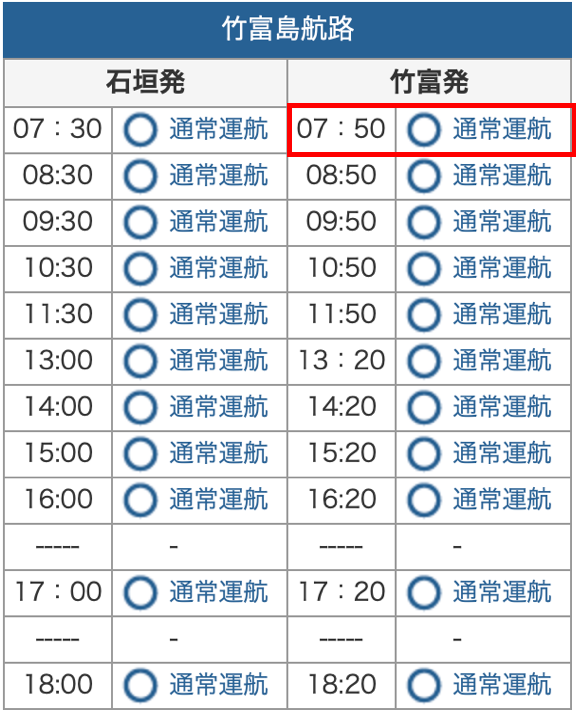
\includegraphics[keepaspectratio, scale=0.5]{pic/anei_sample_data.png}
 \caption{安栄観光\cite{anei}の航路便運航状況}
 \label{anei_label}
\end{figure}

\begin{figure}[H]
 \centering
 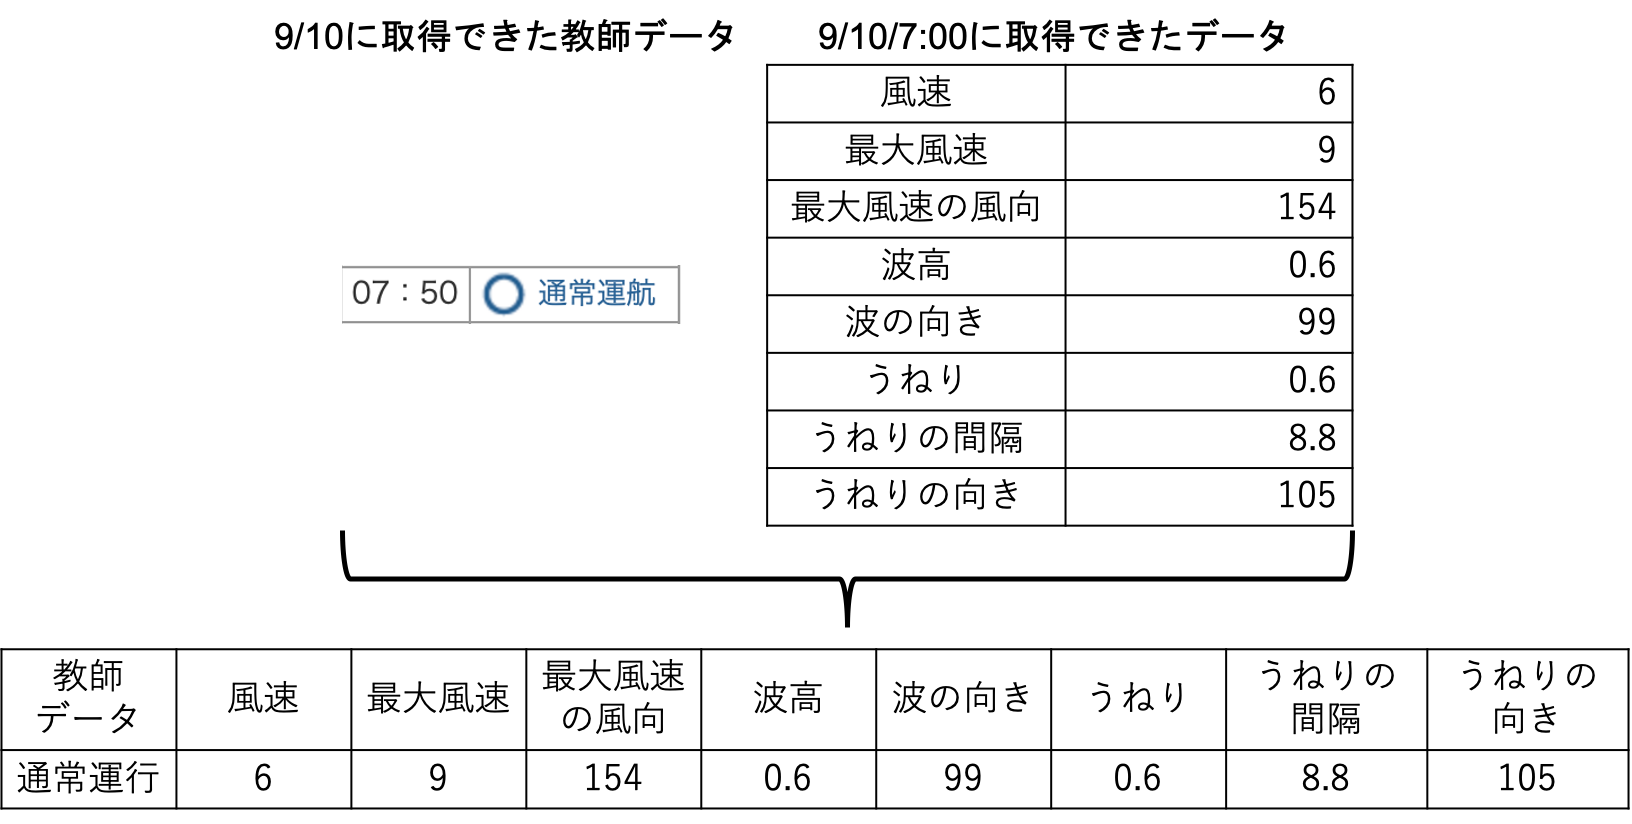
\includegraphics[keepaspectratio, scale=0.3]{pic/value_dataset.png}
 \caption{数値データの作成例}
 \label{value_data}
\end{figure}

\begin{figure}[H]
 \centering
 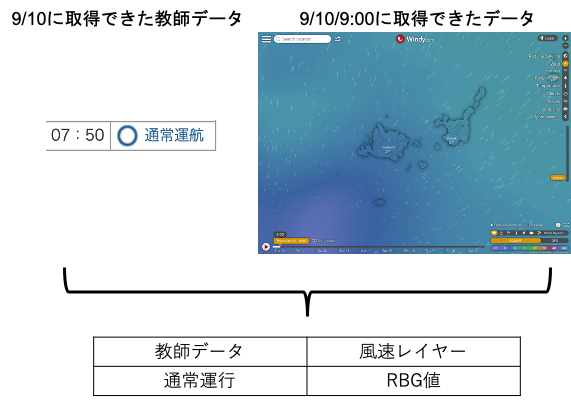
\includegraphics[keepaspectratio, scale=0.3]{pic/wind_speed_data.png}
 \caption{風速画像データの作成例}
 \label{wind_img_data}
\end{figure}

\begin{figure}[H]
 \centering
 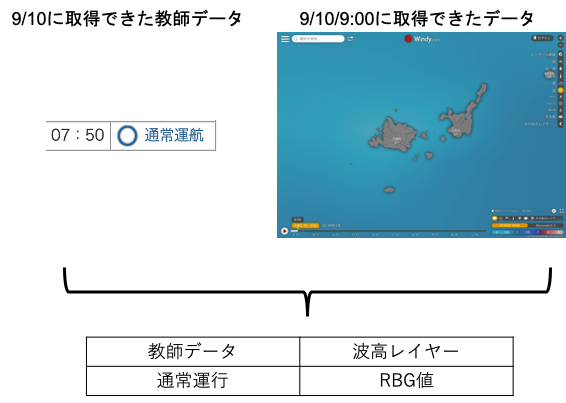
\includegraphics[keepaspectratio, scale=0.3]{pic/wave_height_data.png}
 \caption{波高画像データの作成例}
 \label{wave_value_data}
\end{figure}

\subsection{運航状況の分類手法}
本研究では教師あり学習の分類問題として機械学習モデルを適用する。数値データセットではLightGBMを用い、画像データセットでは、CNNを使用する。
\subsection{学習モデル}
実験に使用したデータは大まかに2020年8月から2021年1月までの期間に取得できたものとなる。
学習モデルは航路に特化させるために航路ごとにデータセットを分けて学習を行うことで7航路あるうちのそれぞれに出発港が2つあるため$7\times2=14$個のモデルとなる。さらに、データを教師データの当日から$9=n$日前までの特徴量をスライドさせ当日のデータから当日の予測、n日前のデータからn日後の予測を行うためにモデルを分割した。モデルを分けて作成したためモデルの総数は$14\times10=140$とし、数値データは図\ref{value_flow}となる。また画像データではさらに風速レイヤー、波高レイヤーで別々のデータセットのため$140\times2=280$個のモデルがあり、図\ref{img_flow}となる。

\begin{figure}[H]
 \centering
 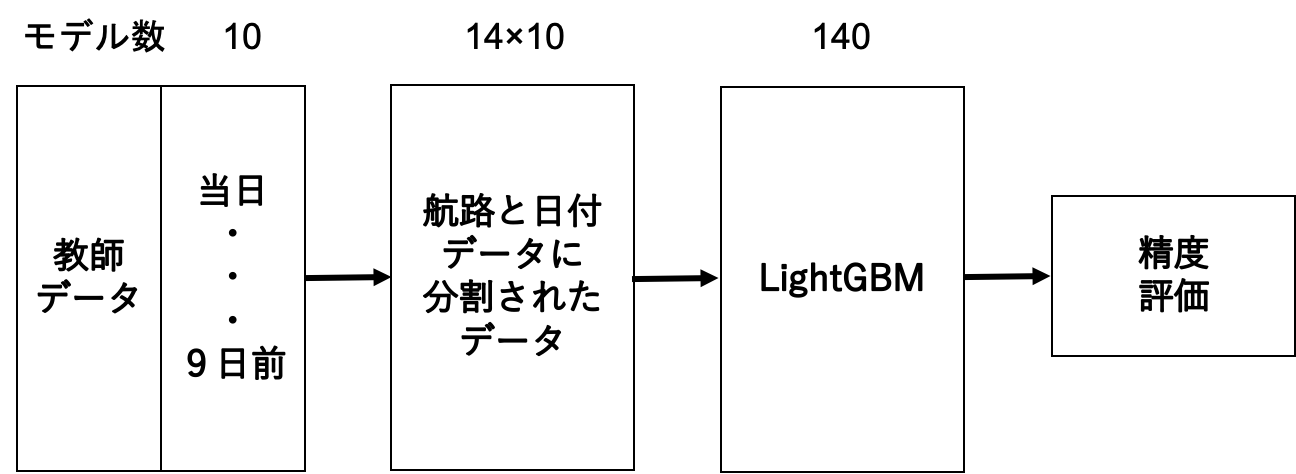
\includegraphics[keepaspectratio, scale=0.3]{pic/value_flow.png}
 \caption{数値データの学習フロー}
 \label{value_flow}
\end{figure}

\begin{figure}[H]
 \centering
 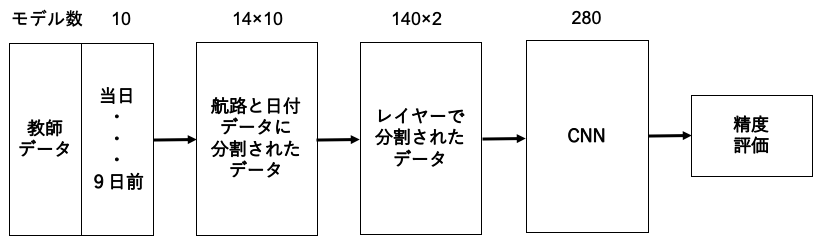
\includegraphics[keepaspectratio, scale=0.3]{pic/img_flow.png}
 \caption{画像データの学習フロー}
 \label{img_flow}
\end{figure}

\section{実験}
\section{数値データによる結果}
数値データを用いた精度(正解率・適合率・再現率・F値)を表\ref{value_hatoma}、表\ref{value_kurosima}に示す。また、西表大原航路、小浜航路、竹富航路では欠航データが無く精度が100\%となったので省く、波照間航路や西表上原航路は表\ref{value_hatoma}のような傾向と似ている結果となったため省く。
\begin{table}[H]
  \begin{center}
    \caption{鳩間島航路-鳩間発}
    \begin{tabular}{|c|r|r|r|r|} \hline
   &正解率 & 適合率 & 再現率 & F値 \\ \hline
      当日&0.868 &0.933 &0.778 &0.848 \\ \hline
     1日前 & 0.816 & 0.875 & 0.737 & 0.800 \\ \hline
      2日前 & 0.816 & 0.929 & 0.684 & 0.788 \\ \hline
      3日前 & 0.649 & 0.636 & 0.737 & 0.683 \\ \hline 
      4日前 & 0.757 & 0.737 & 0.778 & 0.757 \\ \hline 
      5日前 & 0.639 & 0.667 & 0.556 & 0.667 \\ \hline 
      6日前 & 0.722 & 0.833 & 0.556 & 0.667 \\ \hline 
      7日前 & 0.583 & 0.562 & 0.529 & 0.545 \\ \hline 
      8日前 & 0.714 & 0.733 & 0.647 & 0.688 \\ \hline 
      9日前 & 0.629 & 0.625 & 0.588 & 0.606 \\ \hline 
          
    \end{tabular}    
    \label{value_hatoma}
  \end{center}
\end{table}

\begin{table}[H]
  \begin{center}
    \caption{黒島航路-黒島発}
    \begin{tabular}{|c|r|r|r|r|} \hline
   &正解率 & 適合率 & 再現率 & F値 \\ \hline
      当日 & 1.000 & 1.000 & 1.000 & 1.000 \\ \hline
     1日前 & 0.987 & 0.000& 0.000 & 0.000 \\ \hline
      2日前 & 1.000 & 1.000 & 1.000 & 1.000 \\ \hline
      3日前 & 0.986 & 0.000 & 0.000 & 0.000 \\ \hline 
      4日前 & 1.000 & 0.000 & 0.000 & 0.000 \\ \hline 
      5日前 & 0.986 & 0.000 & 0.000 & 0.000 \\ \hline 
      6日前 & 0.986 & 0.000 & 0.000 & 0.000 \\ \hline 
      7日前 & 0.986 & 0.000 & 0.000 & 0.000 \\ \hline 
      8日前 & 1.000 & 1.000 & 1.000 & 1.000 \\ \hline 
      9日前 & 0.986 & 0.000 & 0.000 & 0.000 \\ \hline 
    \end{tabular}    
    \label{value_kurosima}
  \end{center}
\end{table}

\section{画像データによる結果}
画像データの波高レイヤーデータを用いた精度(正解率・適合率・再現率・F値)を表\ref{img_wave_hateruma}、表\ref{img_wave_hatoma}、表\ref{img_wave_taketomi}に示す。また、小浜島航路、黒島航路、西表大原航路は表\ref{img_wave_taketomi}と同様の結果が出力されたため省く、西表航路は表\ref{img_wave_hatoma}と傾向が似ているため省く。

\begin{table}[H]
  \begin{center}
    \caption{波高レイヤー(波照間航路-波照発)}
    \begin{tabular}{|c|r|r|r|r|} \hline
   &正解率 & 適合率 & 再現率 & F値 \\ \hline
      当日&0.796 &0.643 &0.643 &0.643 \\ \hline
     1日前 & 0.833 & 0.857 & 0.462 & 0.600 \\ \hline
      2日前 & 0.723 & 0.000 & 0.000 & 0.000 \\ \hline
      3日前 & 0.723 & 0.000 & 0.000 & 0.000 \\ \hline 
      4日前 & 0.756 & 0.000 & 0.000 & 0.000 \\ \hline 
      5日前 & 0.778 & 0.000 & 0.000 & 0.000 \\ \hline 
      6日前 & 0.773 & 0.000 & 0.000 & 0.000 \\ \hline 
      7日前 & 0.773 & 0.000 & 0.000 & 0.000 \\ \hline 
      8日前 & 0.773 & 0.000 & 0.000 & 0.000 \\ \hline 
      9日前 & 0.767 & 0.000 & 0.000 & 0.000 \\ \hline 
    \end{tabular}    
    \label{img_wave_hateruma}
  \end{center}
\end{table}

\begin{table}[H]
  \begin{center}
    \caption{波高レイヤー(鳩間島航路-鳩間発)}
    \begin{tabular}{|c|r|r|r|r|} \hline
   &正解率 & 適合率 & 再現率 & F値 \\ \hline
      当日 & 0.882 & 0.929 & 0.812 & 0.867 \\ \hline
     1日前 & 0.818 & 0.917 & 0.688 & 0.786 \\ \hline
      2日前 & 0.727 & 0.818 & 0.562 & 0.667 \\ \hline
      3日前 & 0.562 & 0.545 & 0.400 & 0.462 \\ \hline 
      4日前 & 0.594 & 0.538 & 0.500 & 0.519 \\ \hline 
      5日前 & 0.645 & 0.615 & 0.571 & 0.593 \\ \hline 
      6日前 & 0.613 & 0.600 & 0.429 & 0.500 \\ \hline 
      7日前 & 0.581 & 0.545 & 0.429 & 0.480 \\ \hline 
      8日前 & 0.700 & 0.647 & 0.786 & 0.710 \\ \hline 
      9日前 & 0.667 & 0.667 & 0.571 & 0.615 \\ \hline 
    \end{tabular}    
    \label{img_wave_hatoma}
  \end{center}
\end{table}

\begin{table}[H]
  \begin{center}
    \caption{波高レイヤー(竹富航路-竹富発)}
    \begin{tabular}{|c|r|r|r|r|} \hline
   &正解率 & 適合率 & 再現率 & F値 \\ \hline
      当日 & 0.990 & 0.000 & 0.000 & 0.000 \\ \hline
     1日前 & 0.979 & 0.000 & 0.000 & 0.000 \\ \hline
      2日前 & 0.974 & 0.000 & 0.000 & 0.000 \\ \hline
      3日前 & 0.973 & 0.000 & 0.000 & 0.000 \\ \hline 
      4日前 & 0.972 & 0.000 & 0.000 & 0.000 \\ \hline 
      5日前 & 0.972 & 0.000 & 0.000 & 0.000 \\ \hline 
      6日前 & 0.977 & 0.000 & 0.000 & 0.000 \\ \hline 
      7日前 & 0.989 & 0.000 & 0.000 & 0.000 \\ \hline 
      8日前 & 0.994 & 0.000 & 0.000 & 0.000 \\ \hline 
      9日前 & 0.994 & 0.000 & 0.000 & 0.000 \\ \hline 
    \end{tabular}    
    \label{img_wave_taketomi}
  \end{center}
\end{table}

画像データの風速レイヤーデータを用いた精度(正解率・適合率・再現率・F値)を表\ref{img_wind_hateruma}、表\ref{img_wind_iriue}に示す。また、小浜島航路、黒島航路、西表大原航路は表\ref{img_wave_taketomi}と同様の結果が出力されたため省く、鳩間島航路は表\ref{img_wind_iriue}と傾向が似ているため省く。

\begin{table}[H]
  \begin{center}
    \caption{風速レイヤー(波照間航路-波照発)}
    \begin{tabular}{|c|r|r|r|r|} \hline
   &正解率 & 適合率 & 再現率 & F値 \\ \hline
      当日&0.776 &0.579 &0.786 &0.667 \\ \hline
     1日前 & 0.812 & 0.750 & 0.462 & 0.571 \\ \hline
      2日前 & 0.729 & 0.000 & 0.000 & 0.000 \\ \hline
      3日前 & 0.723 & 0.000 & 0.000 & 0.000 \\ \hline 
      4日前 & 0.756 & 0.000 & 0.000 & 0.000 \\ \hline 
      5日前 & 0.778 & 0.000 & 0.000 & 0.000 \\ \hline 
      6日前 & 0.773 & 0.000 & 0.000 & 0.000 \\ \hline 
      7日前 & 0.773 & 0.000 & 0.000 & 0.000 \\ \hline 
      8日前 & 0.750 & 0.000 & 0.000 & 0.000 \\ \hline 
      9日前 & 0.767 & 0.000 & 0.000 & 0.000 \\ \hline 
    \end{tabular}    
    \label{img_wind_hateruma}
  \end{center}
\end{table}

\begin{table}[H]
  \begin{center}
    \caption{風速レイヤー(西表上原航路-西表上原発)}
    \begin{tabular}{|c|r|r|r|r|} \hline
   &正解率 & 適合率 & 再現率 & F値 \\ \hline
      当日 & 0.846 & 0.863 & 0.786 & 0.822 \\ \hline
     1日前 & 0.803 & 0.971 & 0.589 & 0.733 \\ \hline
      2日前 & 0.708 & 0.769 & 0.536 & 0.632 \\ \hline
      3日前 & 0.619 & 0.610 & 0.463 & 0.526 \\ \hline 
      4日前 & 0.696 & 0.684 & 0.531 & 0.598 \\ \hline 
      5日前 & 0.649 & 0.610 & 0.510 & 0.556 \\ \hline 
      6日前 & 0.598 & 0.562 & 0.367 & 0.444 \\ \hline 
      7日前 & 0.527 & 0.429 & 0.180 & 0.254 \\ \hline 
      8日前 & 0.709 & 0.630 & 0.902 & 0.742 \\ \hline 
      9日前 & 0.697 & 0.638 & 0.755 & 0.692 \\ \hline 
    \end{tabular}    
    \label{img_wind_iriue}
  \end{center}
\end{table}


\section{考察}
数値データでは、散布図により特徴量と予測ラベルの分布を示すことで、モデルの重要視している特徴量を発見できた。予測精度の悪いモデルをでは、特徴量の分布に運航時と欠航時の差異がみられない。これらは教師ラベルと特徴量の取得時間のラグがあることに起因すると考えられる。波高、風速画像ではモデルの出力した予測と入力した画像、トレーニングした画像を比較することで、その航路のモデルにおける画像と教師ラベルの関係性、特徴を解析することができた。性能が極端に低いモデルではトレーニングに使用した画像において、教師ラベルと画像の特徴に規則性がほぼ無いために、画像の特徴を捉えられなかったと考えられる。風速、波高の画像どちらもモデルに対しての影響が似ていた。これは船舶の欠航が波高の高さ、風速の大きさによって決定するためであると考えられる。また、画像モデルにおいて欠航データが十分にある航路では、8日前モデルからは評価指標が上昇した。これは本研究で扱った八重山諸島の周辺の気象画像において周期性があると考察できる。
\\ これらの考察より欠航予測のための数値データ、画像データの特徴抽出は時系列を考慮したデータが望ましく、つまり予測に周期性を加味できればより高い精度の予測ができるだろう。
\section{結論}
本研究では船舶の運航状況が当日にしか公表されないという問題を機械学習を用い、比較的安易に入手可能な気象状況の値や気象予報図を適用し数日先までを予測する実験を実施した。画像、数値データどちらも9日先までの予測実験を行い、数値用いた予測では特徴量と教師ラベルとの関係を明らかにすることで、学習モデルが重要視している特徴を確認することができた。特徴量の分散をみることで運航データと欠航データとの特徴量の相関を確認し、予測を行うことにおいて重要な特徴量を確認することができた。画像を用いた予測では航路ごとの入力画像を確認することで、どのような画像がモデルに対して影響を与えているかを示した。また、画像分類では鳩間島、西表上原、小浜島航路において当日から7日前モデルまでは評価指標が減少する傾向にあったが8日前モデルから上昇することを発見した。数値、画像データを時系列的に扱うことで特徴の変遷を保持することができると考えられる。

\thispagestyle{fancy}
\begin{thebibliography}{9}

\bibitem{earth}IPCC, de Coninck, H., A. Revi, M. Babiker, P. Bertoldi, M. Buckeridge, A. Cartwright, W. Dong, J. Ford, S. Fuss, J.-C. Hourcade, D. Ley, R. Mechler, P. Newman, A. Revokatova, S. Schultz, L. Steg, and T. Sugiyama, 2018: Strengthening and Implementing the Global Response. In: Global Warming of 1.5°C. An IPCC Special Report on the impacts of global warming of 1.5°C above pre-industrial levels and related global greenhouse gas emission pathways, in the context of strengthening the global response to the threat of climate change, sustainable development, and efforts to eradicate poverty [MassonDelmotte,V., P. Zhai, H.-O. P\"{o}rtner, D. Roberts, J. Skea, P.R. Shukla, A. Pirani, W. Moufouma-Okia, C. P\'{e}an, R. Pidcock, S. Connors, J.B.R. Matthews, Y. Chen, X. Zhou, M.I. Gomis, E. Lonnoy, T. Maycock, M. Tignor, and T. Waterfield (eds.)]. 
\bibitem{stan}安栄観光,安全管理規定,旅客船. \\ \url{http://www.aneikankou.co.jp/res/pc/pdf/company/legal/anzenkanri5.pdf} \\最終閲覧日:2020/9/14
\bibitem{Related-Research1} 笹 健児,一寺田 大介,永井 紀彦,河合 弘泰,``船体運動と沿岸波浪に基づくフェリー欠航の判断基準に関する検討'',日本航海学会論文集, 120号, pp.99-106, 2009.
\bibitem{anei} 安栄観光. http://www.aneikankou.co.jp/ \\最終閲覧日:2021/1/30
\bibitem{windy}windy.com. \url{https://www.windy.com/} \\最終閲覧日:2021/1/30

\end{thebibliography}
\end{document}
